\documentclass[tikz,border=10pt]{standalone}
\usetikzlibrary{positioning,arrows.meta}
\definecolor{eventFill}{HTML}{FFE0B2}
\definecolor{eventBorder}{HTML}{FB8C00}
\definecolor{subjectFill}{HTML}{C8E6C9}
\definecolor{subjectBorder}{HTML}{4CAF50}
\definecolor{observerFill}{HTML}{E1BEE7}
\definecolor{observerBorder}{HTML}{9C27B0}

\begin{document}
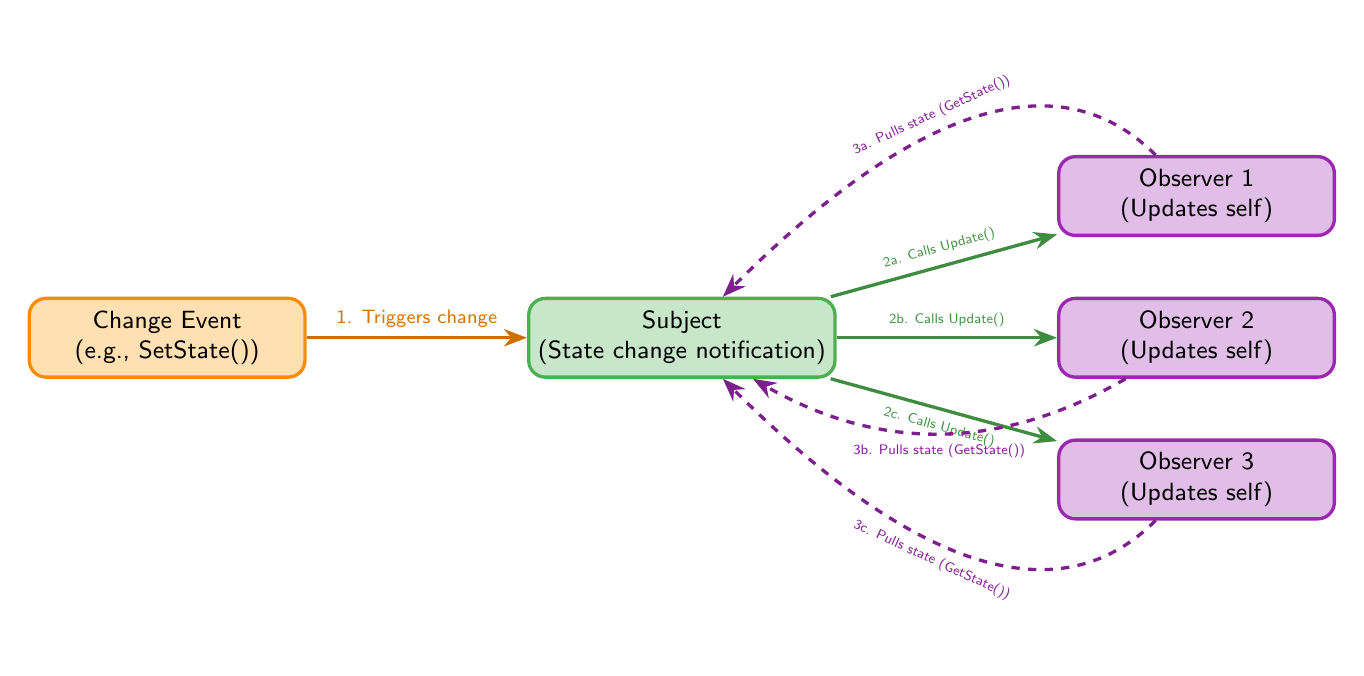
\begin{tikzpicture}[
    block/.style={
        rectangle, draw,
        minimum width=3.5cm, minimum height=1.0cm,
        align=center,
        text centered, rounded corners=6pt,
        line width=1.2pt, font=\sffamily\small
    },
    arrow/.style={-{Stealth[scale=1.0]}, line width=1.2pt}
]
  % Nodes
  \node[block, fill=eventFill, draw=eventBorder] (event) {Change Event\\(e.g., SetState())};
  
  \node[block, fill=subjectFill, draw=subjectBorder, right=2.8cm of event] (subject) {Subject\\(State change notification)};
  
  % Stack of 3 Observers
  \node[block, fill=observerFill, draw=observerBorder, right=2.8cm of subject, yshift=1.8cm] (obs1) {Observer 1\\(Updates self)};
  \node[block, fill=observerFill, draw=observerBorder, right=2.8cm of subject] (obs2) {Observer 2\\(Updates self)};
  \node[block, fill=observerFill, draw=observerBorder, right=2.8cm of subject, yshift=-1.8cm] (obs3) {Observer 3\\(Updates self)};

  % Event to Subject
  \draw[arrow, draw=eventBorder!80!black] (event) -- (subject) 
      node[midway, above, font=\sffamily\scriptsize, text=eventBorder!85!black] {1. Triggers change};
  
  % Notifications (Forward edges)
  \draw[arrow, draw=subjectBorder!80!black] (subject) -- (obs1)
      node[midway, above, sloped, font=\sffamily\tiny, text=subjectBorder!85!black] {2a. Calls Update()};
  \draw[arrow, draw=subjectBorder!80!black] (subject) -- (obs2)
      node[midway, above, font=\sffamily\tiny, text=subjectBorder!85!black] {2b. Calls Update()};
  \draw[arrow, draw=subjectBorder!80!black] (subject) -- (obs3)
      node[midway, below, sloped, font=\sffamily\tiny, text=subjectBorder!85!black] {2c. Calls Update()};
      
  % Pull state updates (Backward dashed edges with curved lines to avoid overlaps)
  \draw[arrow, draw=observerBorder!80!black, dashed] (obs1) to[out=135,in=45] 
      node[midway, above, sloped, font=\sffamily\tiny, text=observerBorder!85!black] {3a. Pulls state (GetState())} (subject);
      
  \draw[arrow, draw=observerBorder!80!black, dashed] (obs2) to[out=210,in=330] 
      node[midway, below, font=\sffamily\tiny, text=observerBorder!85!black] {3b. Pulls state (GetState())} (subject);
      
  \draw[arrow, draw=observerBorder!80!black, dashed] (obs3) to[out=225,in=315] 
      node[midway, below, sloped, font=\sffamily\tiny, text=observerBorder!85!black] {3c. Pulls state (GetState())} (subject);

\end{tikzpicture}
\end{document}
